\section{ Responsive Design }

\subsection{ Choosing a Framwork }
With regards to responsive design, there are a number of frameworks, one can
choose with regards to creating a web app. The following are quite popular:
\begin{enumerate}
  \item Foundation
  \item Bootstrap
  \item Semantic UI
\end{enumerate}

However, the above for a grid system tend to be overkill in my opinion.
Specifically, the direction many UI web app tend to head, is that it will only
be used on Desktop. For mobile and tablet, there will be a separate Android and
IOS app created. In addition, due to the nature of angulars component
architecture, the use of ready made components, containers for apps, are the
only thing which will actually have specific media queries.

It is strongly suggested that your own super lightweight grid is created, or
used. I think it is important to keep in mind that most grid systems can be
limited to 500 lines of code, or less. I personally prefer to use Skeleton
\footnote{http://getskeleton.com/\#grid}. However, I am in the process of
creating my own grid system using css-grid. (need to get back to this one).

Alternatively, creating our own grid system is also advantageous. That is the
direction that will make sense in any enterprise app. Generally, in any business
setting, from the business side they will decide on having a unique look and
feel. Setting up something for the app that works.

\subsection{ Breakpoints }
The reccomended architecture for a design language system is material design.
First, it really is the largest design system. Second, think about it this way.
Which design language would you rather choose, the one created by the company
that uses the same front end framework that you are using, or the one created
by the company, not using the same front end framework you are using? I 100%
realized that this logic can be flawed. However, the company that we are talking
about is Google, so... yeah.

Now you might be thinking, that a design language system, is front end framework
agnostic. However, I would like to make the following point. A design language
system, is then built into a component library. If a design language is not
built with a particular front end framework in mind, the odds of it being
built into a robust component library, are slim. Angular Material Components is
so robust, is almost turns not using Material Design as your design language as
a sin.

\subsubsection{ Official Material Design Breakpoints }
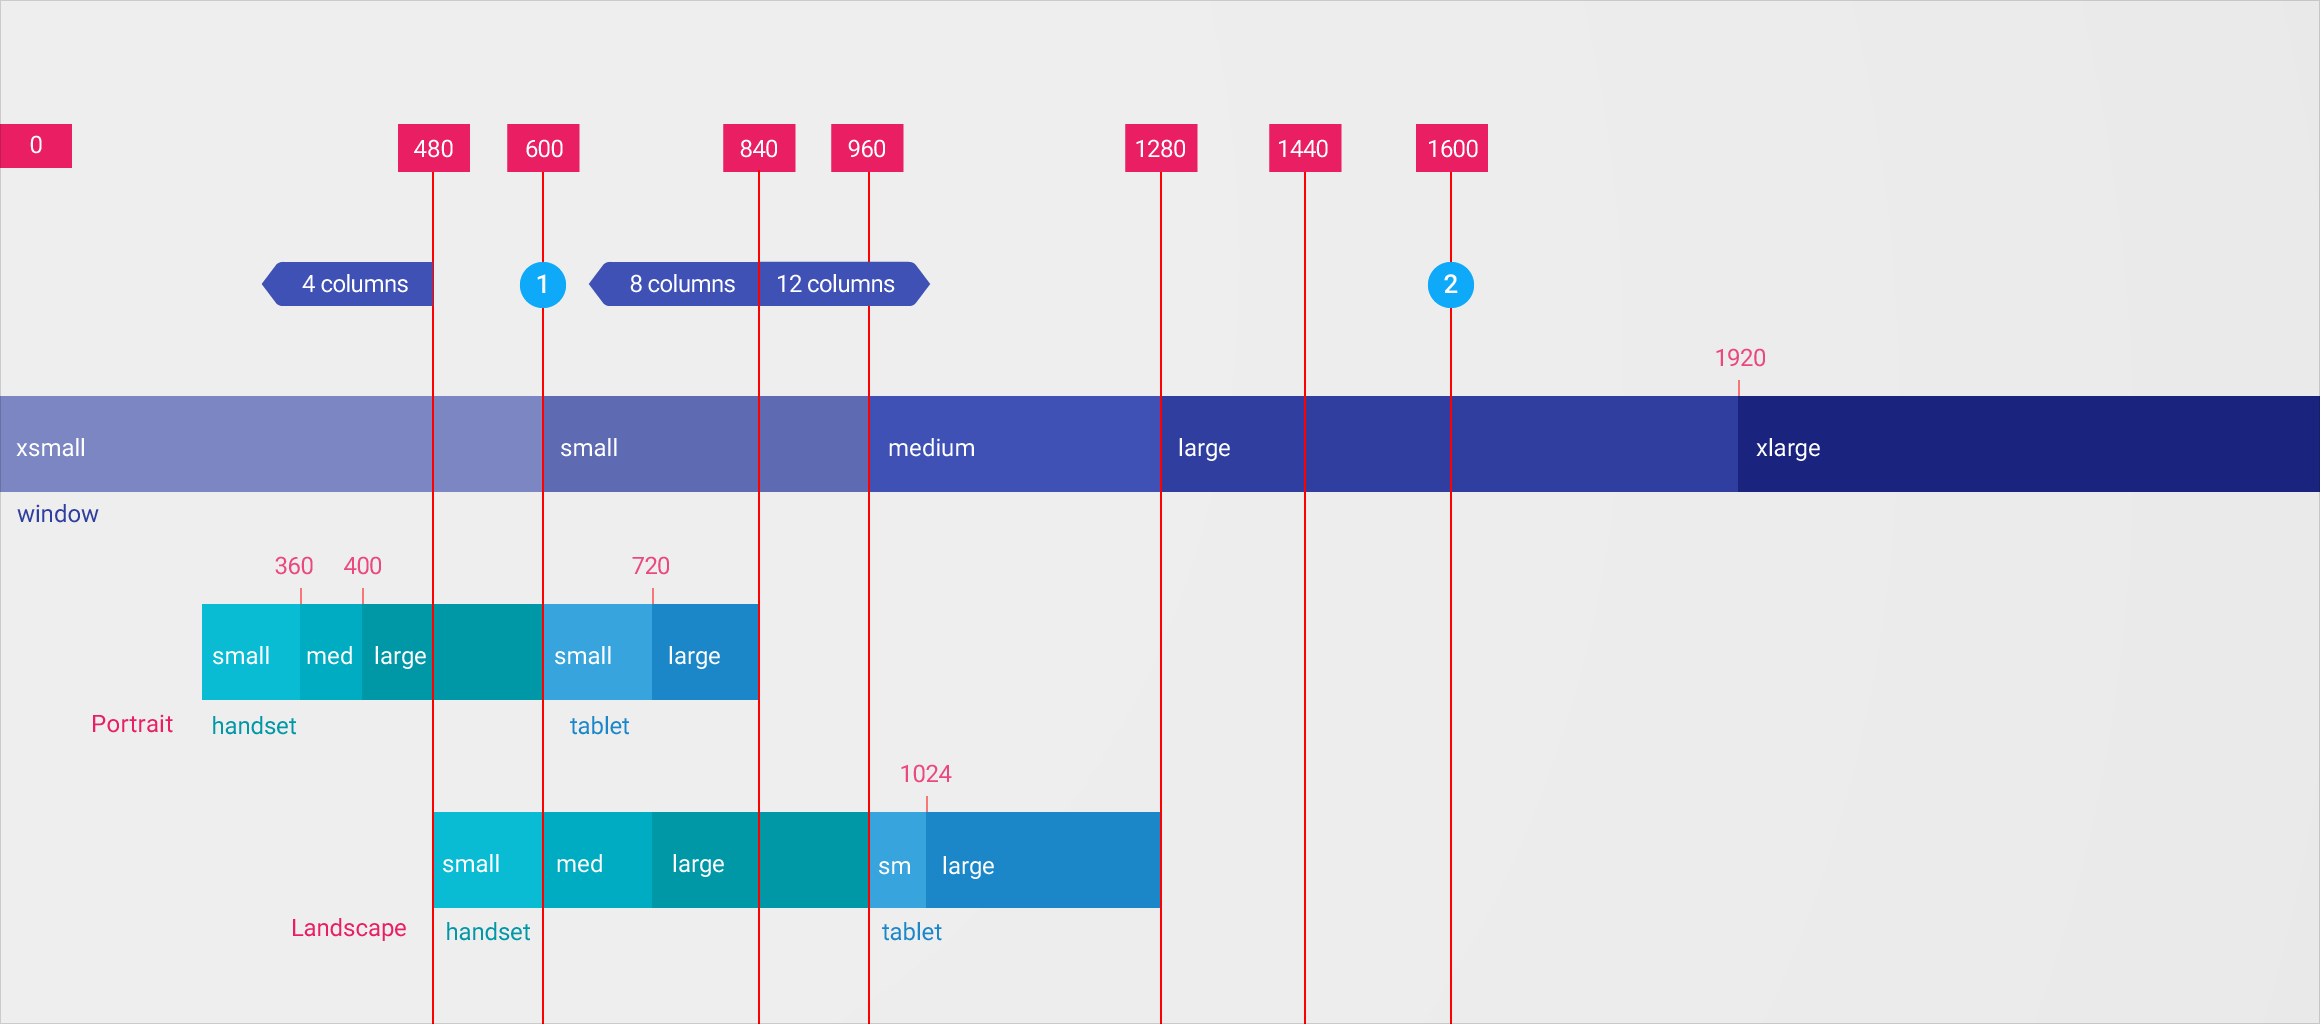
\includegraphics[scale=0.15]{responsive/layout-adaptive-breakpoints}

\subsubsection{ Choosing Four Specific Breakpoints }
Even within an enterprise setting, using all the breakpoints specified within
the Material Design specification can be quite a bit. We recommend using the
following breakpoints:

\begin{enumerate}
  \item 400px[Mobile Large - Portrait]
  \item 720px[Tablet Large - Portrait + Mobile Large - Landscape]
  \item 1024px[Tablet Large - Landscape]
  \item 1424px[Desktop Large](16p below 1440 to accommodate for gutter space)
\end{enumerate}

\subsubsection{ Build Media Query Function }
Per conventions, it is reccomended that all items relating to the DLS be
specified with regards to functions. That way, we have a way of making sure
that nothing deviates from the design language system.

We will be creating an ill-ui folder and ill.scss file) in our lib folder, to
hold all all of our app's .scss files. In addition, we will be creating an
 \_ill-breakpoints.scss file, to be imported in our ill-ui.scss file. We will be
creating the following in our app:

\begin{verbatim}
  // Testing
\end{verbatim}
